% IEEE conference paper -- compile with pdfLaTeX (e.g. Overleaf). Tables/figures in generated/ are
% produced from the experiment result files by:  python -m ml.experiments.paper_assets
\documentclass[conference]{IEEEtran}
\IEEEoverridecommandlockouts
\usepackage{cite}
\usepackage{amsmath,amssymb,amsfonts}
\usepackage{graphicx}
\usepackage{booktabs}
\usepackage{xcolor}
\usepackage{tikz}
\usetikzlibrary{arrows.meta,positioning,fit,backgrounds,calc}
\usepackage[hidelinks]{hyperref}

% Marks content that depends on experiments that have not finished. Remove all before submission.
\newcommand{\pending}[1]{\textcolor{red}{\textbf{[#1]}}}

\begin{document}

\title{Leakage-Aware Detection of Diffusion-Era Facial Deepfakes with an Explainable Forensic Analysis Platform}

\author{
\IEEEauthorblockN{Author One\textsuperscript{1}, Author Two\textsuperscript{1}}
\IEEEauthorblockA{\textsuperscript{1}Department of Computer Science and Engineering, \textit{College Name}, City, Country\\
\{author1, author2\}@college.edu}
}

\maketitle

\begin{abstract}
Detectors for manipulated and AI-generated images are frequently reported with near-perfect accuracy, yet such figures can be inflated by data leakage, dataset shortcuts and the absence of robustness testing. We present a leakage-aware evaluation of two ImageNet-pretrained convolutional detectors, ResNet-50 and EfficientNet-B0, on the DeepFakeFace (DFF) dataset of diffusion-based face inpainting, InsightFace face swaps and Stable Diffusion text-to-image faces, integrated into an open, explainable forensic analysis platform. A data audit of DFF revealed 165 sets (344 images) of byte-identical real photographs filed under different identities, 84 of which would span an identity-based split, and tens of thousands of cross-identity near-duplicates; we therefore merge leakage groups across (near-)duplicates before splitting. With validation-selected thresholds, ResNet-50 reaches 95.12\% accuracy (95\% CI 94.7--95.6) and 0.990 ROC-AUC on 9{,}000 held-out test images, and EfficientNet-B0 reaches 94.38\% and 0.988. Face swaps are markedly harder (82.6--89.3\% detection) than diffusion inpainting or text-to-image fakes (95.6--99.4\%). Robustness testing shows strong fragility: JPEG quality 50 reduces accuracy to 74--76\% and Gaussian noise ($\sigma{=}15$) to 55--62\%, with most fakes then classified as real. We additionally document that every DFF fake is a 512$\times$512 JPEG while no real image is, a potential shortcut that we control for. The platform exposes calibrated decision thresholds, Grad-CAM explanations, measured image forensics and per-image robustness probing through a web interface, and all code and evaluation outputs are reproducible.
\end{abstract}

\begin{IEEEkeywords}
deepfake detection, AI-generated images, image forensics, data leakage, robustness, Grad-CAM, convolutional neural networks
\end{IEEEkeywords}

\section{Introduction}
Diffusion models and face-swapping toolkits can now produce photorealistic faces at scale, which complicates the verification of images shared online. Learned detectors based on convolutional neural networks (CNNs) are a common response \cite{wang2020cnn,rossler2019ff}, and many report accuracies close to 100\%. Such numbers can, however, overstate real-world reliability for three reasons: (i) leakage between training and test data, for instance when the same photograph appears under several identities; (ii) dataset shortcuts, such as systematic differences in image size or compression between real and fake classes \cite{grommelt2024fake}; and (iii) evaluation only on clean images, although shared media is routinely recompressed, resized and filtered.

This paper makes the following contributions:
\begin{itemize}
\item A leakage-aware protocol for the DeepFakeFace (DFF) dataset \cite{song2023dff}: a data audit (exact and perceptual duplicates, format and size statistics) and identity groups merged across (near-)duplicates before splitting.
\item A controlled comparison of ResNet-50 \cite{he2016resnet} and EfficientNet-B0 \cite{tan2019efficientnet} with validation-only threshold selection, grouped-bootstrap confidence intervals, per-manipulation analysis and a ten-condition robustness suite.
\item An open forensic analysis platform (FastAPI/PyTorch backend, React frontend) that serves the trained detectors with Grad-CAM \cite{selvaraju2017gradcam} explanations, measured image forensics and per-image robustness probing, while explicitly communicating uncertainty.
\end{itemize}

\section{Related Work}
\textit{Face manipulation detection.} FaceForensics++ \cite{rossler2019ff} established CNN baselines for face swaps and reenactment and showed that compression strongly affects detection. DFF \cite{song2023dff} extends this setting to diffusion-based manipulations and reports degraded generalisation across generators. \textit{AI-generated image detection.} Wang et al.\ \cite{wang2020cnn} showed that a ResNet-50 trained on one GAN generalises surprisingly well with suitable augmentation, while Ojha et al.\ \cite{ojha2023universal} and Corvi et al.\ \cite{corvi2023diffusion} studied generalisation to diffusion models. GenImage \cite{zhu2023genimage} provides a million-scale benchmark across eight generators. \textit{Frequency artefacts.} Up-sampling layers leave spectral traces \cite{durall2020upconv,frank2020frequency}, motivating frequency-domain features. \textit{Dataset bias.} Grommelt et al.\ \cite{grommelt2024fake} demonstrated that JPEG-compression and size differences between classes in GenImage allow detectors to succeed for spurious reasons. Our work applies this critical perspective to facial deepfakes and couples it with an explainable, deployable system.

\section{Methodology}

\subsection{System architecture}
Fig.~\ref{fig:system} summarises the platform. Uploaded images are validated by content (magic bytes and a full decode; size and pixel limits), never by file extension. A model registry loads installed checkpoints once and caches them. Each checkpoint embeds its architecture, preprocessing configuration, class order and decision threshold, so that inference reproduces the evaluation pipeline exactly. For every analysis the backend returns the fake score, the thresholded label, a Grad-CAM overlay, a Fourier spectrum and measured file properties (format, EXIF with sensitive fields redacted, JPEG quantisation-table quality estimate). Results are stored in SQLite and exported as PDF reports. Two separate tracks, AI-generated images and facial deepfakes, use separate models and protocols.

\begin{figure}[!t]
\centering
\resizebox{\columnwidth}{!}{%
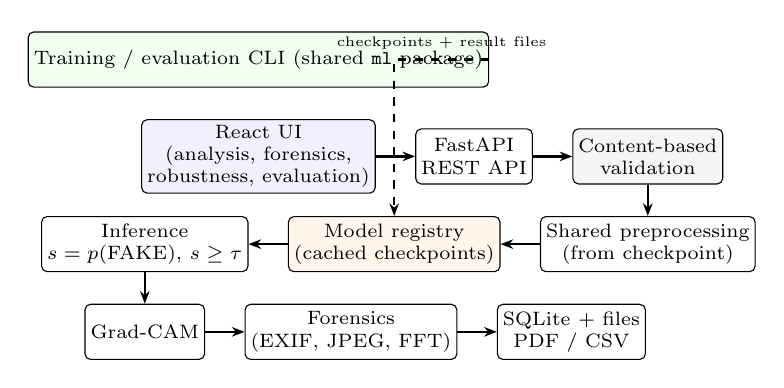
\begin{tikzpicture}[
  node distance=4mm and 5mm,
  box/.style={draw, rounded corners=2pt, align=center, font=\scriptsize, minimum height=7mm, inner sep=2pt, fill=white},
  grp/.style={draw, dashed, rounded corners=3pt, inner sep=3pt},
  arr/.style={-{Stealth[length=1.6mm]}, thick}]
\node[box, fill=blue!6] (ui) {React UI\\(analysis, forensics,\\robustness, evaluation)};
\node[box, right=of ui] (api) {FastAPI\\REST API};
\node[box, right=of api, fill=gray!8] (val) {Content-based\\validation};
\node[box, below=of val] (pre) {Shared preprocessing\\(from checkpoint)};
\node[box, left=of pre, fill=orange!8] (reg) {Model registry\\(cached checkpoints)};
\node[box, left=of reg] (inf) {Inference\\$s=p(\mathrm{FAKE})$, $s\ge\tau$};
\node[box, below=of inf] (cam) {Grad-CAM};
\node[box, right=of cam] (for) {Forensics\\(EXIF, JPEG, FFT)};
\node[box, right=of for] (db) {SQLite + files\\PDF / CSV};
\node[box, above=of ui, fill=green!6] (ml) {Training / evaluation CLI (shared \texttt{ml} package)};
\draw[arr] (ui) -- (api);
\draw[arr] (api) -- (val);
\draw[arr] (val) -- (pre);
\draw[arr] (pre) -- (reg);
\draw[arr] (reg) -- (inf);
\draw[arr] (inf) -- (cam);
\draw[arr] (cam) -- (for);
\draw[arr] (for) -- (db);
\draw[arr, dashed] (ml.east) -| node[pos=0.25, above, font=\tiny]{checkpoints + result files} (reg.north);
\end{tikzpicture}}
\caption{Platform architecture. Training and evaluation share the same \texttt{ml} package as the API, so preprocessing is identical at training, evaluation and inference time.}
\label{fig:system}
\end{figure}

\subsection{Detector architecture}
Fig.~\ref{fig:detector} shows the detector. A backbone $f_\theta$ (ResNet-50 or EfficientNet-B0, initialised with torchvision ImageNet weights \cite{deng2009imagenet}) maps an input $x\in\mathbb{R}^{3\times224\times224}$ to a pooled feature vector $h=f_\theta(x)$ ($d=2048$ or $1280$). The ImageNet classifier is replaced by dropout and a linear layer producing logits $z=Wh+b\in\mathbb{R}^2$, with class 0 = REAL and class 1 = FAKE. The fake score is
\begin{equation}
s(x)=\mathrm{softmax}(z)_1=\frac{e^{z_1}}{e^{z_0}+e^{z_1}},
\end{equation}
and an image is labelled FAKE iff $s(x)\ge\tau$. The score is not calibrated as a probability. An optional frequency branch (used in the ablation) computes the standardised centred log-magnitude spectrum $\log(1+|\mathcal{F}(Y)|)$ of the luminance $Y$ inside the network and encodes it with four strided convolutions into a 128-dimensional vector that is concatenated with $h$. ResNet-50 and EfficientNet-B0 detectors have 23.51\,M and 4.01\,M parameters; the frequency branch adds 0.24\,M.

\begin{figure}[!t]
\centering
\resizebox{\columnwidth}{!}{%
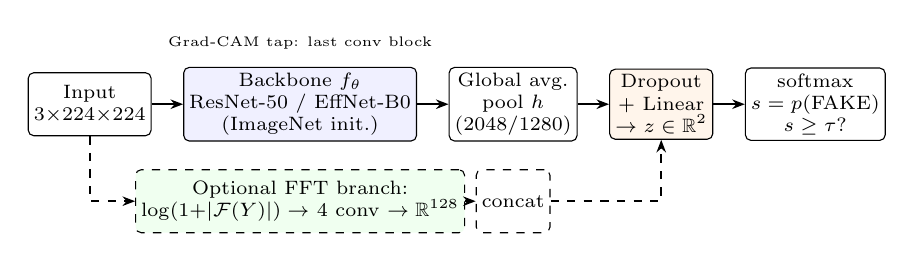
\begin{tikzpicture}[
  node distance=3.5mm and 4mm,
  box/.style={draw, rounded corners=2pt, align=center, font=\scriptsize, minimum height=8mm, inner sep=2pt},
  arr/.style={-{Stealth[length=1.6mm]}, thick}]
\node[box] (in) {Input\\$3{\times}224{\times}224$};
\node[box, right=of in, fill=blue!6, minimum width=24mm] (bb) {Backbone $f_\theta$\\ResNet-50 / EffNet-B0\\(ImageNet init.)};
\node[box, right=of bb] (gap) {Global avg.\\pool $h$\\($2048/1280$)};
\node[box, right=of gap, fill=orange!8] (head) {Dropout\\+ Linear\\$\to z\in\mathbb{R}^2$};
\node[box, right=of head] (sm) {softmax\\$s=p(\mathrm{FAKE})$\\$s\ge\tau$?};
\node[box, below=of bb, fill=green!6, dashed, minimum width=24mm] (fft) {Optional FFT branch:\\$\log(1{+}|\mathcal{F}(Y)|)\to$ 4 conv $\to\mathbb{R}^{128}$};
\node[box, below=of gap, dashed] (cat) {concat};
\node[font=\tiny, align=center, above=1mm of bb] (gc) {Grad-CAM tap: last conv block};
\draw[arr] (in) -- (bb);
\draw[arr] (bb) -- (gap);
\draw[arr] (gap) -- (head);
\draw[arr] (head) -- (sm);
\draw[arr, dashed] (in.south) |- (fft.west);
\draw[arr, dashed] (fft) -- (cat);
\draw[arr, dashed] (cat) -| (head.south);
\end{tikzpicture}}
\caption{Detector architecture. The ImageNet head is replaced by a two-class head. The decision threshold $\tau$ is selected on the validation split.}
\label{fig:detector}
\end{figure}

\subsection{Preprocessing and shortcut control}
Images are decoded, converted to RGB and resized to $224\times224$, then normalised with ImageNet statistics. The identical transform, stored in each checkpoint, is used for validation, testing and API inference. As a control against size and format shortcuts, an optional source normalisation resizes every image (both classes) to a short side of 256, centre-crops it and re-encodes it as JPEG at quality 90 before the model transform.

\subsection{Training}\label{sec:training}
Models are fine-tuned with cross-entropy, AdamW \cite{loshchilov2019adamw} (weight decay $10^{-4}$; learning rate $10^{-4}$ for ResNet-50 and $3{\times}10^{-4}$ for EfficientNet-B0), a one-epoch linear warm-up followed by cosine decay, gradient clipping at 1.0, batch sizes 48/64, and float16 automatic mixed precision on an NVIDIA RTX~4060 Laptop GPU (8\,GB). Augmentation consists of horizontal flips and random crops (80--100\% area). Training uses a fixed, seeded class-balanced random subset of 30{,}000 training images (15{,}000 per class); model and threshold selection use a balanced 6{,}000-image validation subset. Training runs for at most 8 epochs with early stopping on validation ROC-AUC (patience 3). The checkpoint with the best validation ROC-AUC is kept, and $\tau$ is chosen on the validation split by maximising Youden's $J=\mathrm{TPR}-\mathrm{FPR}$ \cite{youden1950index}. The test split is never used for model or threshold selection. Software: PyTorch 2.14 \cite{paszke2019pytorch}, torchvision 0.29, scikit-learn 1.9; seed 42.

\subsection{Explainability}
Grad-CAM \cite{selvaraju2017gradcam} computes $L^c=\mathrm{ReLU}(\sum_k\alpha_k^cA^k)$ with $\alpha_k^c=\frac{1}{Z}\sum_{i,j}\partial z_c/\partial A^k_{ij}$ at the last convolutional block (a $7\times7$ grid at $224^2$ input) for the predicted class $c$. We treat the maps as qualitative evidence only.

\subsection{Evaluation}
We report accuracy, per-class precision and recall, macro-F1, ROC-AUC and confusion matrices (FAKE as the positive class), plus single-image latency (batch size 1, warm-up excluded, CUDA-synchronised). 95\% confidence intervals use a percentile bootstrap with 1{,}000 resamples over leakage groups rather than images \cite{efron1993bootstrap}, which respects the correlation between a real image and the fakes derived from it. Robustness is measured at the unchanged threshold under JPEG compression (quality 90/70/50), downscaling ($\times0.5$, $\times0.25$, resized back), Gaussian blur ($\sigma=1,2$) and Gaussian noise ($\sigma=5,15$ on the 0--255 scale).

\section{Datasets and Data Audit}
\textit{DeepFakeFace (DFF)} \cite{song2023dff} contains 30{,}000 real celebrity images from IMDB-WIKI \cite{rothe2018imdbwiki} and, for each, three fakes: Stable Diffusion inpainting, an InsightFace \cite{deng2019arcface} face swap, and Stable Diffusion v1.5 \cite{rombach2022ldm} text-to-image generation (120{,}000 images). Each fake is stored under the same file name as its source image, which we use as the initial leakage group.

Our audit (Table~\ref{tab:audit}) found no missing or corrupted files, but 165 sets (344 images) of byte-identical real photographs filed under different identifiers (no set mixes real and fake labels). With an identity-only split (v1), 84 of these sets and 19{,}949 cross-identity near-duplicate pairs (64-bit dHash, Hamming distance $\le4$) would span splits. We therefore merged leakage groups connected by near-duplicates (Hamming $\le2$, union-find) before a 70/15/15 group-level split (v2, Table~\ref{tab:dataset}). The merge reduced 30{,}000 groups to 18{,}511. It can over-merge similar but distinct faces, which only makes the split more conservative. The audit also showed that \emph{all} 90{,}000 fakes are 512$\times$512 JPEGs, whereas no real image is 512$	imes$512: in a random sample of 3{,}000 real images the median short side is 440\,px (5th percentile 223\,px), and 1{,}048 real images are PNG, GIF or MPO files. A classifier could therefore exploit resampling or format cues. We quantify this with the shortcut-control variant (Sec.~\ref{sec:results}). The test set is a class-balanced random sample of 4{,}500 real and 4{,}500 fake test images.

For the AI-generated-image track we use a random subset of the official GenImage \cite{zhu2023genimage} test images: 1{,}000 real (ImageNet) and 1{,}000 generated images for each of eight generators (ADM, BigGAN, GLIDE, Midjourney, SD v1.4, SD v1.5, VQDM, Wukong), re-split 70/15/15 after the same duplicate merging (47 merges).

\input{generated/tab_audit.tex}
\input{generated/tab_dataset.tex}

\section{Results}\label{sec:results}

\subsection{Facial deepfake detection}
Table~\ref{tab:main_dff} reports test performance. ResNet-50 achieves 95.12\% accuracy and 0.990 ROC-AUC, and EfficientNet-B0 achieves 94.38\% and 0.988. The confidence intervals of the two models overlap for ROC-AUC, so with a single training seed we do not claim a significant difference between architectures. The validation-selected thresholds differ substantially ($\tau=0.194$ vs.\ $0.638$), which illustrates that a fixed threshold of 0.5 is not appropriate for uncalibrated scores. EfficientNet-B0 trades lower fake recall (92.3\%) for higher real recall (96.4\%) at 60\% of ResNet-50's training time per epoch (57\,s vs.\ 95\,s) and with 5.9$\times$ fewer parameters. Both models run in under 10\,ms per image. Fig.~\ref{fig:roc} shows the ROC curves and Table~\ref{tab:confusion} the confusion matrices.

\input{generated/tab_main_dff.tex}
\input{generated/tab_confusion.tex}

\begin{figure}[!t]
\centering
\includegraphics[width=\columnwidth]{generated/fig_roc_dff.pdf}
\caption{ROC curves on the DFF test split (inset: low-FPR region).}
\label{fig:roc}
\end{figure}

\subsection{Per-manipulation analysis}
Table~\ref{tab:per_method_dff} shows that diffusion-generated content is detected almost perfectly (text-to-image 98.9--99.4\%, inpainting 95.6--98.3\%), whereas InsightFace swaps are the main source of errors (82.6\% for EfficientNet-B0, 89.3\% for ResNet-50). Unlike text-to-image and inpainting, a face swap preserves most of the original photograph, leaving less synthetic content for the detector to find.

\input{generated/tab_per_method_dff.tex}

\subsection{Robustness}
Table~\ref{tab:robust_dff} and Fig.~\ref{fig:robust} reveal pronounced fragility. Mild JPEG compression (quality 90) is harmless, but quality 50 reduces accuracy to 76.0\% (ResNet-50) and 74.2\% (EfficientNet-B0), mostly by misclassifying real images as fake. Downscaling and blur also lower real-image recall (e.g.\ 69.1\% for ResNet-50 at $\times0.25$), while fakes remain detected. Additive Gaussian noise has the opposite effect: at $\sigma=15$ fake recall collapses to 10.1\% (ResNet-50) and 24.7\% (EfficientNet-B0), and nearly every image is labelled real. Together these asymmetric failure modes indicate that both models rely heavily on fine-grained high-frequency statistics rather than semantic facial evidence. This has a direct practical consequence: images that have been recompressed or noised by social-media pipelines cannot be judged reliably.

\input{generated/tab_robust_dff.tex}

\begin{figure}[!t]
\centering
\includegraphics[width=\columnwidth]{generated/fig_robust_dff.pdf}
\caption{Test accuracy under perturbations (fixed threshold). Each point is an independent condition.}
\label{fig:robust}
\end{figure}

\subsection{Explainability}
Fig.~\ref{fig:gradcam} shows Grad-CAM maps for randomly sampled true and false positives and negatives of ResNet-50. For fakes and many real images the maps concentrate on the face region, while some false positives highlight clothing or background. The real-image class also contains non-portrait images (e.g.\ a postage stamp), which reflects label noise in the source data. False negatives receive very low fake scores ($s\approx0$), so errors are made with high confidence. We stress that such maps are qualitative and do not establish that the model uses forensically meaningful evidence.

\begin{figure}[!t]
\centering
\includegraphics[width=\columnwidth]{generated/fig_gradcam_dff.png}
\caption{Grad-CAM (predicted class) for ResNet-50 on DFF test images: true positives, true negatives, false positives and false negatives; $s$ is the fake score ($\tau=0.194$).}
\label{fig:gradcam}
\end{figure}

\subsection{Shortcut control and generalisation}
To test whether the size/format difference is exploited, we retrained EfficientNet-B0 with the source normalisation applied to both classes. On the validation split it reached 95.43\% accuracy and 0.991 ROC-AUC (vs.\ 94.90\% and 0.990 without normalisation), i.e.\ equalising size and JPEG encoding did \emph{not} reduce performance, which suggests that this difference is not the main cue used by the detector. \pending{Test-set results for this variant (third row of Table~\ref{tab:main_dff}) and the leave-one-manipulation-out experiment (Table~\ref{tab:cross_manip}) are still being computed; update this paragraph with the test numbers.}

\input{generated/tab_cross_manip.tex}

\subsection{AI-generated image detection}
\pending{GenImage experiments (baseline comparison over two seeds, leave-one-generator-out, and RGB vs.\ RGB+FFT vs.\ JPEG-augmentation ablation) have not been run yet. Tables~\ref{tab:main_genimage}--\ref{tab:ablation} will be populated automatically. Note the known JPEG bias of GenImage \cite{grommelt2024fake}: real images are JPEG and generated images are PNG.}

\input{generated/tab_main_genimage.tex}
\input{generated/tab_cross_gen.tex}
\input{generated/tab_ablation.tex}

\section{Discussion and Limitations}
High in-distribution accuracy on DFF (95\%) coexists with severe sensitivity to common post-processing and with systematic differences in size and format between classes. We therefore recommend that detector results always be reported together with a data audit, leakage-aware splits, threshold provenance and a robustness suite. Our study has the following limitations: a single training seed per configuration (confidence intervals capture test-set sampling variability, not training variability); a single dataset per track; ImageNet-pretrained CNN backbones only; and, for DFF, near-duplicate merging based on a coarse perceptual hash. The detector outputs a score, not proof. The platform presents every prediction with its threshold, an uncertainty disclaimer and measured forensic context, and it performs no identity recognition.

\section{Conclusion}
We presented a leakage-aware evaluation of CNN detectors for diffusion-era facial deepfakes, integrated into an explainable forensic analysis platform. ResNet-50 and EfficientNet-B0 reach 95.1\% and 94.4\% test accuracy on DFF after duplicate-aware splitting, but face swaps remain harder, and accuracy drops to 55--76\% under strong compression or noise. A data audit uncovered cross-identity duplicates and a systematic size/format difference between classes that would otherwise go unnoticed. Future work includes multi-seed and cross-dataset evaluation, robustness-oriented training, and calibrated uncertainty estimates.

\section*{Data and Code Availability}
DFF is available from its authors under its stated license; GenImage from its official release. Manifests, configurations, result files and the generator for all tables and figures in this paper are part of the project repository.

\begin{thebibliography}{00}
\bibitem{rossler2019ff} A. R\"ossler, D. Cozzolino, L. Verdoliva, C. Riess, J. Thies, and M. Nie{\ss}ner, ``FaceForensics++: Learning to detect manipulated facial images,'' in \textit{Proc. IEEE/CVF Int. Conf. Comput. Vis. (ICCV)}, 2019, pp. 1--11.
\bibitem{song2023dff} H. Song, S. Huang, Y. Dong, and W.-W. Tu, ``Robustness and generalizability of deepfake detection: A study with diffusion models,'' arXiv:2309.02218, 2023.
\bibitem{zhu2023genimage} M. Zhu \textit{et al.}, ``GenImage: A million-scale benchmark for detecting AI-generated image,'' in \textit{Adv. Neural Inf. Process. Syst. (NeurIPS) Datasets and Benchmarks Track}, 2023.
\bibitem{he2016resnet} K. He, X. Zhang, S. Ren, and J. Sun, ``Deep residual learning for image recognition,'' in \textit{Proc. IEEE Conf. Comput. Vis. Pattern Recognit. (CVPR)}, 2016, pp. 770--778.
\bibitem{tan2019efficientnet} M. Tan and Q. V. Le, ``EfficientNet: Rethinking model scaling for convolutional neural networks,'' in \textit{Proc. Int. Conf. Mach. Learn. (ICML)}, 2019, pp. 6105--6114.
\bibitem{selvaraju2017gradcam} R. R. Selvaraju, M. Cogswell, A. Das, R. Vedantam, D. Parikh, and D. Batra, ``Grad-CAM: Visual explanations from deep networks via gradient-based localization,'' in \textit{Proc. IEEE Int. Conf. Comput. Vis. (ICCV)}, 2017, pp. 618--626.
\bibitem{wang2020cnn} S.-Y. Wang, O. Wang, R. Zhang, A. Owens, and A. A. Efros, ``CNN-generated images are surprisingly easy to spot\ldots for now,'' in \textit{Proc. IEEE/CVF Conf. Comput. Vis. Pattern Recognit. (CVPR)}, 2020, pp. 8695--8704.
\bibitem{ojha2023universal} U. Ojha, Y. Li, and Y. J. Lee, ``Towards universal fake image detectors that generalize across generative models,'' in \textit{Proc. IEEE/CVF Conf. Comput. Vis. Pattern Recognit. (CVPR)}, 2023, pp. 24480--24489.
\bibitem{corvi2023diffusion} R. Corvi, D. Cozzolino, G. Zingarini, G. Poggi, K. Nagano, and L. Verdoliva, ``On the detection of synthetic images generated by diffusion models,'' in \textit{Proc. IEEE Int. Conf. Acoust., Speech Signal Process. (ICASSP)}, 2023.
\bibitem{durall2020upconv} R. Durall, M. Keuper, and J. Keuper, ``Watch your up-convolution: CNN based generative deep neural networks are failing to reproduce spectral distributions,'' in \textit{Proc. IEEE/CVF Conf. Comput. Vis. Pattern Recognit. (CVPR)}, 2020, pp. 7890--7899.
\bibitem{frank2020frequency} J. Frank, T. Eisenhofer, L. Sch\"onherr, A. Fischer, D. Kolossa, and T. Holz, ``Leveraging frequency analysis for deep fake image recognition,'' in \textit{Proc. Int. Conf. Mach. Learn. (ICML)}, 2020, pp. 3247--3258.
\bibitem{grommelt2024fake} P. Grommelt, L. Weiss, F.-J. Pfreundt, and J. Keuper, ``Fake or JPEG? Revealing common biases in generated image detection datasets,'' arXiv:2403.17608, 2024.
\bibitem{rothe2018imdbwiki} R. Rothe, R. Timofte, and L. Van Gool, ``Deep expectation of real and apparent age from a single image without facial landmarks,'' \textit{Int. J. Comput. Vis.}, vol. 126, no. 2--4, pp. 144--157, 2018.
\bibitem{deng2019arcface} J. Deng, J. Guo, N. Xue, and S. Zafeiriou, ``ArcFace: Additive angular margin loss for deep face recognition,'' in \textit{Proc. IEEE/CVF Conf. Comput. Vis. Pattern Recognit. (CVPR)}, 2019, pp. 4690--4699.
\bibitem{rombach2022ldm} R. Rombach, A. Blattmann, D. Lorenz, P. Esser, and B. Ommer, ``High-resolution image synthesis with latent diffusion models,'' in \textit{Proc. IEEE/CVF Conf. Comput. Vis. Pattern Recognit. (CVPR)}, 2022, pp. 10684--10695.
\bibitem{deng2009imagenet} J. Deng, W. Dong, R. Socher, L.-J. Li, K. Li, and L. Fei-Fei, ``ImageNet: A large-scale hierarchical image database,'' in \textit{Proc. IEEE Conf. Comput. Vis. Pattern Recognit. (CVPR)}, 2009, pp. 248--255.
\bibitem{loshchilov2019adamw} I. Loshchilov and F. Hutter, ``Decoupled weight decay regularization,'' in \textit{Proc. Int. Conf. Learn. Represent. (ICLR)}, 2019.
\bibitem{youden1950index} W. J. Youden, ``Index for rating diagnostic tests,'' \textit{Cancer}, vol. 3, no. 1, pp. 32--35, 1950.
\bibitem{efron1993bootstrap} B. Efron and R. J. Tibshirani, \textit{An Introduction to the Bootstrap}. New York, NY, USA: Chapman \& Hall, 1993.
\bibitem{paszke2019pytorch} A. Paszke \textit{et al.}, ``PyTorch: An imperative style, high-performance deep learning library,'' in \textit{Adv. Neural Inf. Process. Syst. (NeurIPS)}, 2019, pp. 8024--8035.
\end{thebibliography}

\end{document}
